\documentclass{beamer}
\usepackage[section]{placeins}
\usepackage{float}
\usepackage[position=b]{subfig}

\mode<presentation>{
  %   \usetheme{CambridgeUS}      % or try Darmstadt, Madrid, Warsaw, ...
  \usetheme{Frankfurt}
  % \definecolor{mygreen}{cmyk}{0.6,0.168,0.168,0.25}
  % \definecolor{mygreen}{RGB}{84,135,138}

  % \definecolor{myblue}{RGB}{23, 91, 127}
  \definecolor{myblue}{RGB}{24, 71, 160}
  \setbeamercolor{structure}{fg=myblue}
  \usefonttheme{default}
  \setbeamertemplate{navigation symbols}{}
  %\setbeamertemplate[compatibility=false, numbered]{caption}
  \setbeamertemplate{itemize items}[default]
  \setbeamertemplate{enumerate items}[default]
  \defbeamertemplate*{title page}{customized}[1][]{
  \centering
   \begin{beamercolorbox}[rounded=true,shadow=true,leftskip=1cm,colsep*=.75ex]{title}
  \centering
   \usebeamerfont{title}\inserttitle\par
    \end{beamercolorbox}
     \par\medskip\medskip\medskip
     \begin{columns}

     \begin{column}{0.6\textwidth}
        \usebeamerfont{author}\insertauthor\par\medskip\medskip
        \usebeamerfont{institute}\insertinstitute\par\medskip\medskip
        \usebeamerfont{date}\insertdate\par
        % \medskip \medskip \medskip
        \begin{figure}[!htbp]
         \begin{center}
          \subfloat{
            
\includegraphics[width=0.4\columnwidth]{figuras/cnpqLogo.jpg}
          }
          \hspace{1cm}
          \subfloat{
            
\includegraphics[width=0.2\columnwidth]{figuras/capesLogo.png}
          }
        \end{center}
        \end{figure}
      \end{column}
    \begin{column}{0.3\textwidth}
    
\includegraphics[width=\columnwidth]{figuras/brasao_usp_pb}
    \end{column}
    \end{columns}
  }

  \setbeamertemplate{footline}{
    \begin{beamercolorbox}[colsep=1.5pt]{upper separation line foot}
    \end{beamercolorbox}
    \hbox{%
   \begin{beamercolorbox}[wd=0.82\paperwidth, ht=2.5ex, dp=1.125ex, left]{title in head/foot}%
        \usebeamerfont{title in head/foot}\hspace*{2ex}\insertshorttitle
      \end{beamercolorbox}%

      \begin{beamercolorbox}[wd=0.09\paperwidth, ht=2.5ex, dp=1.125ex, center]{title in head/foot}%
        \usebeamerfont{author in head/foot}{\insertshortinstitute }
      \end{beamercolorbox}%

      \begin{beamercolorbox}[wd=0.09\paperwidth, ht=2.5ex, dp=1.125ex, right]{title in head/foot}%
        \usebeamerfont{title in head/foot}\insertframenumber/\inserttotalframenumber\hspace*{2ex}
      \end{beamercolorbox}}
    \begin{beamercolorbox}[colsep=1.5pt]{lower separation line foot}
    \end{beamercolorbox}
  }
}

\makeatletter
\renewcommand{\itemize}[1][]{%
  \beamer@ifempty{#1}{}{\def\beamer@defaultospec{#1}}%
  \ifnum \@itemdepth >2\relax\@toodeep\else
    \advance\@itemdepth\@ne
    \beamer@computepref\@itemdepth% sets \beameritemnestingprefix
    \usebeamerfont{itemize/enumerate \beameritemnestingprefix body}%
    \usebeamercolor[fg]{itemize/enumerate \beameritemnestingprefix body}%
    \usebeamertemplate{itemize/enumerate \beameritemnestingprefix body begin}%
    \list
      {\usebeamertemplate{itemize \beameritemnestingprefix item}}
      {\def\makelabel##1{%
          {%
            \hss\llap{{%
                \usebeamerfont*{itemize \beameritemnestingprefix item}%
                \usebeamercolor[fg]{itemize \beameritemnestingprefix item}##1}}%
          }%
        }%
      }
  \fi%
  \beamer@cramped%
  \justifying% NEW
  %\raggedright% ORIGINAL
  \beamer@firstlineitemizeunskip%
}
\makeatother

\useoutertheme[subsection=false]{miniframes}
\usepackage{etoolbox}
\makeatletter
\patchcmd{\slideentry}{\advance\beamer@xpos by1\relax}{}{}{}
\def\beamer@subsectionentry#1#2#3#4#5{\advance\beamer@xpos by1\relax}%
\makeatother

\usepackage{ragged2e}
\usepackage{lipsum}
\usepackage[sort, numbers]{natbib}
% \usepackage[style=alphabetic]{biblatex}

\usepackage[linesnumbered,ruled,vlined]{algorithm2e}
%\usepackage{algorithm}
\usepackage{algpseudocode}
\SetKwFor{Para}{para}{fa\c{c}a}{fim}
\SetKwFor{ParaCada}{para cada}{fa\c{c}a}{fim}
\SetKwRepeat{DoWhile}{faça}{enquanto}

\usepackage[compatibility=false]{caption}
% \usepackage{subcaption}
\usepackage[brazil]{babel}
\usepackage[utf8x]{inputenc}
\usepackage{setspace}
\usepackage{ragged2e}
\usepackage{graphicx}
\usepackage{amsmath,amsfonts,amssymb}
\usepackage{xcolor}
\usepackage{url}
\usepackage{array}
\usepackage{gensymb}
\usepackage{multicol}
\usepackage[loadonly]{enumitem}
\newlist{arrowlist}{itemize}{1}
\setlist[arrowlist]{label=$\Rightarrow$}
\usepackage{listings}
\newcommand{\fonte}[1]{\caption*{Fonte: #1}}
\newcommand{\fonteminha}{\caption*{Fonte: Elaborado pelo autor.}}

\title[\textbf{Geração de imagens artificiais e quantização aplicadas a problemas de classificação}]{\textbf{Geração de imagens artificiais e quantização aplicadas a problemas de classificação}}
\author{Gabriela Salvador Thumé \\ \vspace{4pt}
        \tiny Orientador: Prof. Dr. Moacir Antonelli Ponti \\ \vspace{4pt}
        \tiny Co-orientador: Prof. Dr. João do Espirito Santo Batista Neto}
\institute[ICMC/USP]{Instituto de Ciências Matemáticas e de Computação \\
Universidade de São Paulo \\ }
\date{29 de abril de 2016}
%%%%%%%%%%%%%%%%%%%%%%%%%%%%%%%%%%%%%%%%%%%%%%%%%%%%%%%%%%%%%%%%%%%%%%%%%%%%%%%
\begin{document}
\setbeamercovered{transparent}
\begin{frame}[plain]
  \maketitle
\end{frame}
%%%%%%%%%%%%%%%%%%%%%%%%%%%%%%%%%%%%%%%%%%%%%%%%%%%%%%%%%%%%%%%%%%%%%%%%%%%%%%%
\begin{frame}[noframenumbering]{Estrutura da Apresentação}
\setstretch{1.2}
% \begin{multicols}{2}
  \tableofcontents
% \end{multicols}
\end{frame}
\section{Introdução}
%%%%%%%%%%%%%%%%%%%%%%%%%%%%%%%%%%%%%%%%%%%%%%%%%%%%%%%%%%%%%%%%%%%%%%%%%%%%%%%
\AtBeginSection[]{
\begin{frame}<beamer>[noframenumbering]{Estrutura da Apresentação}
\setstretch{1.2}
% \begin{multicols}{2}
\tableofcontents[currentsection, sectionstyle=show/shaded,
]
% \tableofcontents[currentsection,currentsubsection, hideothersubsections,
%     sectionstyle=show/shaded,
% ]
% \end{multicols}
\end{frame}
}
%%%%%%%%%%%%%%%%%%%%%%%%%%%%%%%%%%%%%%%%%%%%%%%%%%%%%%%%%%%%%%%%%%%%%%%%%%%%%%%
\begin{frame}{Introdução}
\setstretch{1.2}
\setlength\leftmargini{0em}
\justifying
\begin{itemize}
\item Classificação de imagens;
\pause
\item Extração de características;
\pause
\item Algoritmos de aprendizado de máquina: modelo de representação;
\item Generalização permite classificar novos exemplos;
\pause
\item Características que não são suficientes para a diferenciação entre as classes;
\item Encontrar as características que melhor discriminam as classes.
\end{itemize}
\end{frame}
%-----------------------------------------------------------------------------
\subsection{Motivação}
\begin{frame}[plain]{Motivação}
\begin{figure}
    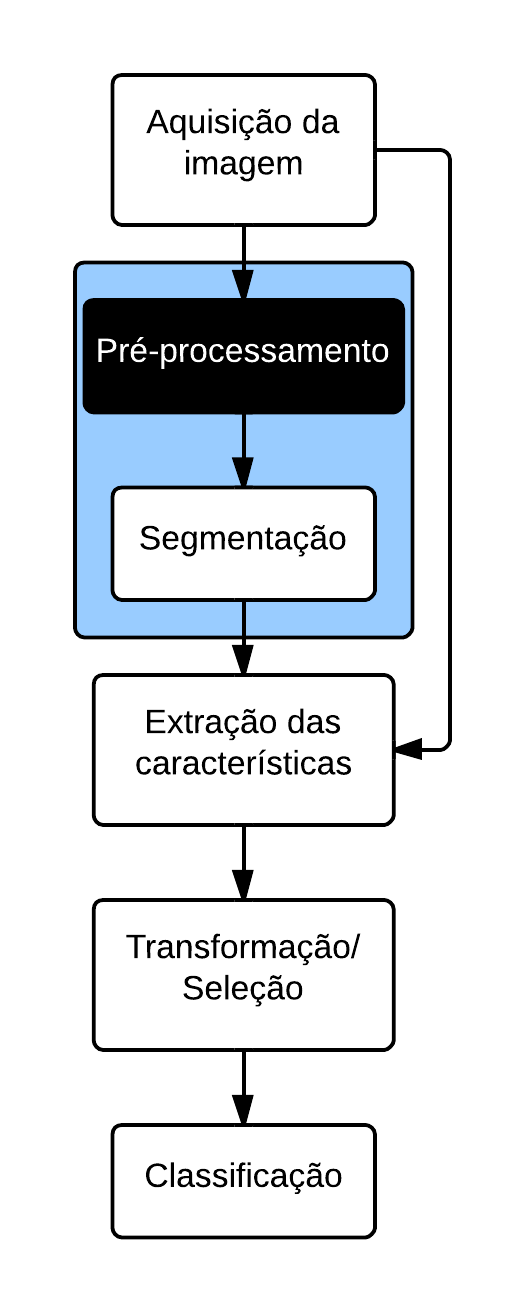
\includegraphics[height=0.9\textheight]{figuras/flow.png}
    \caption{Etapas canônicas do reconhecimento de padrões.}
\end{figure}
\end{frame}
%-----------------------------------------------------------------------------
\begin{frame}{Motivação}
\setstretch{1.2}
\setlength\leftmargini{0em}
\justifying
\begin{itemize}
\item Maior esforço ao operar no espaço de características já obtidas;
\item Transformações do espaço ou sistemas complexos de classificação para lidar com as deficiências das características extraídas;
\item Características que podem ser exploradas além dos métodos clássicos;
\item Investigar métodos de processamento e preparação de imagens antes da extração.
\end{itemize}
\end{frame}
%-----------------------------------------------------------------------------
\begin{frame}{Motivação - Características Latentes}
\setlength\leftmargini{0em}
\justifying
\setstretch{1.2}
\begin{itemize}
\item Justificado o uso de métodos de processamento e preparação de imagens antes da extração;
\item Podem revelar características latentes, não visíveis nas imagens originais;
\item Foco: \emph{revelar características que possam melhor descrever certas classes, utilizando algoritmos sobre as imagens originais.}
\end{itemize}
\end{frame}
%-----------------------------------------------------------------------------
\begin{frame}{Motivação}
\setlength\leftmargini{0em}
\justifying
 \setstretch{1.2}
  \begin{itemize}
\justifying
    \item 98\% de acurácia após pré-processamento e segmentação (Rocha et al., 2010); % frutas
    \item Quantização pode impactar a classificação (Kanan e Cottrell, 2012);
    \item Quantização permite obter vetores de características mais compactos e com maior capacidade de discriminação entre classes (Ponti et al., 2014);
    \item[]  {Continuação.}
  \end{itemize}
\end{frame}
%-----------------------------------------------------------------------------
\begin{frame}{Motivação - Desbalanceamento de classes}
\setlength\leftmargini{0em}
\justifying
% \setstretch{1.2}
  \begin{itemize}
    \item Diferença entre o número de exemplos disponíveis;
    \item Imagens representam eventos importantes mas menos frequentes;
    \item Obstáculo, métodos de transformação do espaço e de
    classificação assumem que a base está balanceada;
    \item Foco: \emph{geração de imagens artificiais a partir do processamento de características das imagens da classe minoritária.}
  \end{itemize}
  \begin{figure}[htbp]
 \begin{center}
   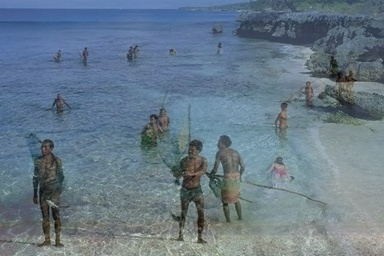
\includegraphics[width=.4\linewidth]{figuras/imagemgerada.jpg}
 \caption{Imagem artificialmente gerada.}
 \end{center}
\end{figure}

\end{frame}
%-----------------------------------------------------------------------------
\subsection{Hipóteses e Objetivos}
\setstretch{1.2}
\setlength\leftmargini{1em}
\justifying
 \begin{frame}{Hipóteses}
  \begin{block}{Métodos de pré-processamento}
    \justifying
    \begin{itemize}
      \item Evidenciar características latentes que aumentem a variância entre as classes, sem aumentar a variância intra-classe;
      \item Melhorar a classificação.
    \end{itemize}
  \end{block}
  \begin{block}{Geração de imagens artificiais}
    \justifying
    \begin{itemize}
      \item Balancear as classes;
      \item Melhorar a acurácia, versus geração de exemplos artificiais no espaço de atributos.
    \end{itemize}
  \end{block}
\end{frame}
%%%%%%%%%%%%%%%%%%%%%%%%%%%%%%%%%%%%%%%%%%%%%%%%%%%%%%%%%%%%%%%%%%%%%%%%%%%%%%%
\begin{frame}{Objetivo Geral}
\setstretch{1.2}
\setlength\leftmargini{1em}
\justifying
  \begin{block}{}
  \justifying
  \emph{Investigar os métodos de pré-processamento para preparar uma coleção de imagens para a extração de características.}

  \vspace{5mm}
  Espera-se obter características latentes e balancear o número de instâncias de diferentes classes.
  \end{block}
\end{frame}
%-----------------------------------------------------------------------------
\begin{frame}{Objetivos Específicos}
% \setstretch{1.2}
\setlength\leftmargini{1em}
\justifying
    \begin{itemize}
      \item Analisar:
        \begin{itemize}
          \item impacto de métodos canônicos na classificação;
          \item aprendizado de bases comportadas por redes de convolução.
        \end{itemize}
      \item Tornar as características latentes visíveis;% com o auxílio dos métodos canônicos e CNN;
      \item Gerar imagens artificiais.
      \pause
        \begin{itemize}
          \item Resultados preliminares;
          % \item Estudo das características latentes encontradas no treinamento da classe minoritária de uma rede de convolução;
          \item Matriz de características aprendida por uma máquina de Boltzmann restrita para verificar a relevância das imagens geradas e as imagens originais.
        \end{itemize}
    \end{itemize}
\end{frame}
%-----------------------------------------------------------------------------
\begin{frame}{Proposta}
\begin{figure}
    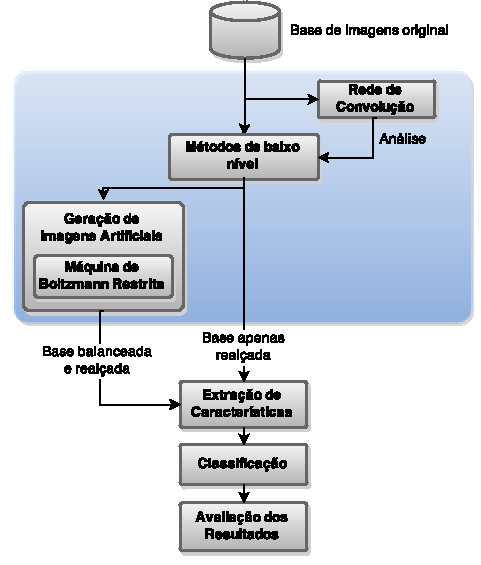
\includegraphics[height=0.75\textheight]{figuras/geral.pdf}
    \caption{Estrutura geral desta pesquisa.}
\end{figure}
\end{frame}
%-----------------------------------------------------------------------------
\section{Contextualização}
\subsection{Pré-processamento}
\begin{frame}{Pré-processamento de Imagens}
\begin{figure}
    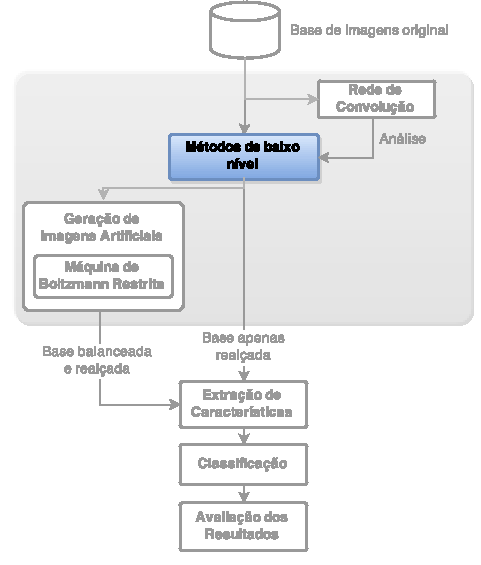
\includegraphics[height=0.75\textheight]{figuras/geral_metodos.pdf}
\end{figure}
\end{frame}
%-----------------------------------------------------------------------------
\begin{frame}{Pré-processamento de Imagens}
\begin{figure}[htbp]
 \begin{center}
   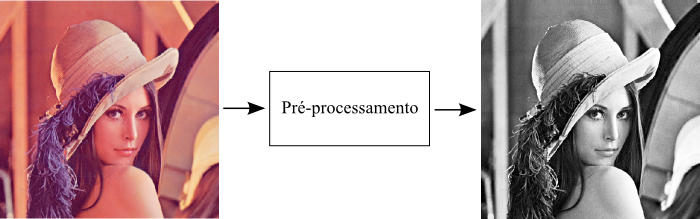
\includegraphics[width=1\linewidth]{figuras/preprocessamento.png}
 \caption{Conversão em escala de cinza, borramento, realce e de equalização de histograma.}
 \end{center}
\end{figure}
\end{frame}
%-----------------------------------------------------------------------------
\begin{frame}{Pré-processamento de Imagens - Convolução}
\setlength\leftmargini{0em}
\justifying
\setstretch{1.2}
\begin{itemize}
    \item Percorre a imagem com um filtro espacial rotacionado em $180\degree$; \\
    \item Cria cada novo pixel com as mesmas coordenadas do centro da vizinhança contendo o valor resultante da filtragem.
\end{itemize}
\begin{figure}[htbp]
 \begin{center}
   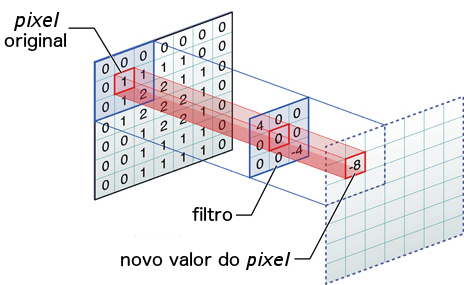
\includegraphics[width=.5\linewidth]{figuras/convolucao.png}
 \caption{Convolução com filtro previamente rotacionado.}
 \end{center}
\end{figure}
\end{frame}
%-----------------------------------------------------------------------------
\begin{frame}{Pré-processamento de Imagens - Convolução}
\begin{figure}[!htbp]
  \begin{center}
  \subfloat[Original]{
    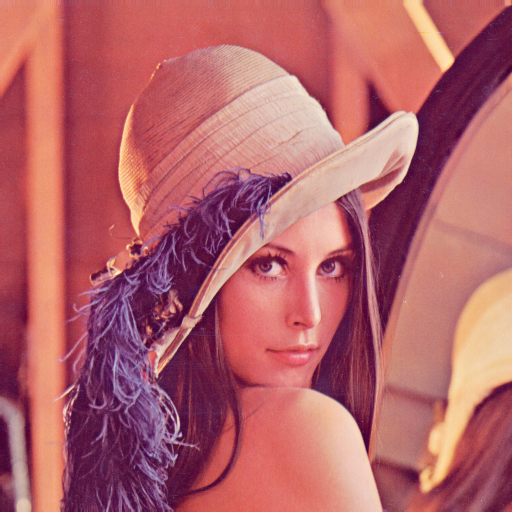
\includegraphics[width=0.5\linewidth]{figuras/original.png}
  }
  \subfloat[Filtragem Gaussiana]{
    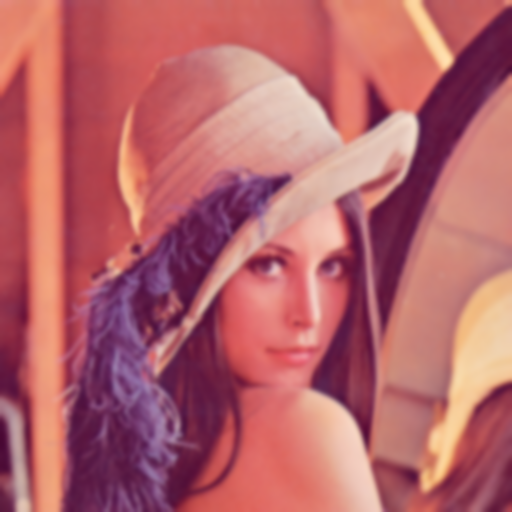
\includegraphics[width=0.5\linewidth]{figuras/blur.png}
  }
  \end{center}
\end{figure}
\end{frame}
%-----------------------------------------------------------------------------
\begin{frame}{Pré-processamento de Imagens - Realce}
\begin{figure}[!htbp]
  \begin{center}
  \subfloat[Original]{
    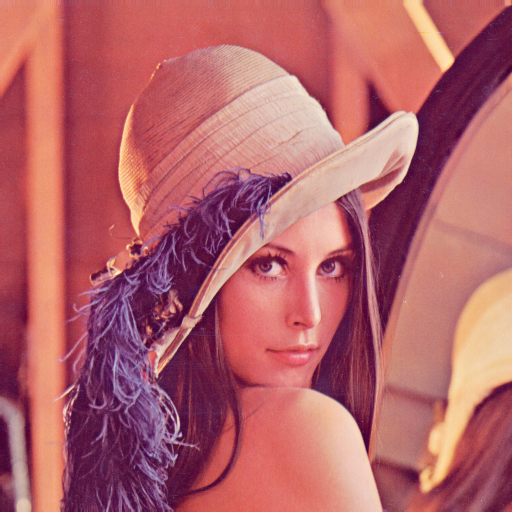
\includegraphics[width=0.5\linewidth]{figuras/original.png}
  }
  \subfloat[Unsharp masking]{
    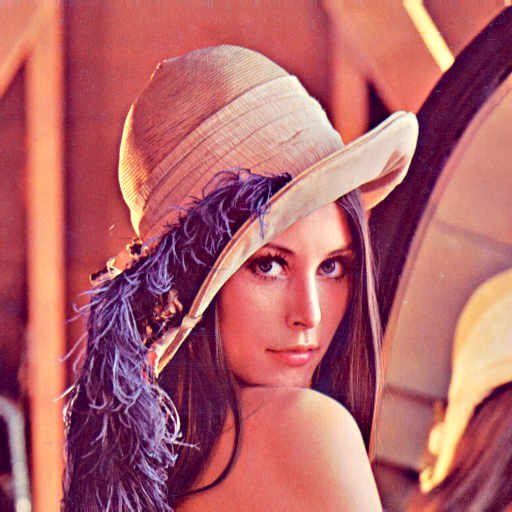
\includegraphics[width=0.5\linewidth]{figuras/unsharpmask.png}
  }
 \end{center}
\end{figure}
\end{frame}
%-----------------------------------------------------------------------------
\begin{frame}{Pré-processamento de Imagens - Quantização}
\begin{figure}[!htbp]
 \begin{center}
  \subfloat[Original]{
    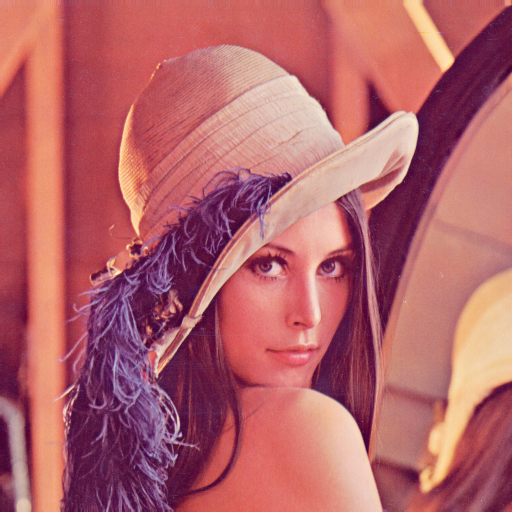
\includegraphics[width=.3\linewidth]{\detokenize{figuras/quantization/Lenna.png}}
  }
  \subfloat[Intensidade']{
    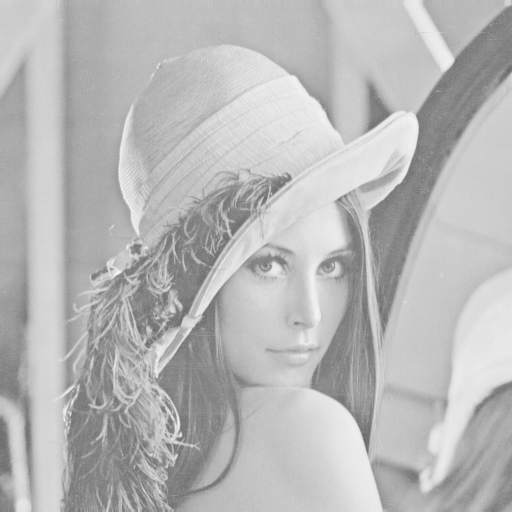
\includegraphics[width=.3\linewidth]{\detokenize{figuras/quantization/Intensity_gray.png}}
    \label{fig:intensidade}
  }
  \subfloat[Gleam]{
    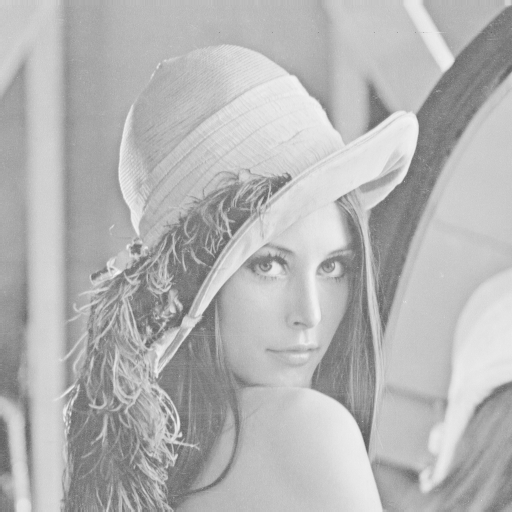
\includegraphics[width=.3\linewidth]{\detokenize{figuras/quantization/Gleam_gray.png}}
    \label{fig:gleam}
  }
  \newline
  \subfloat[Luminância']{
    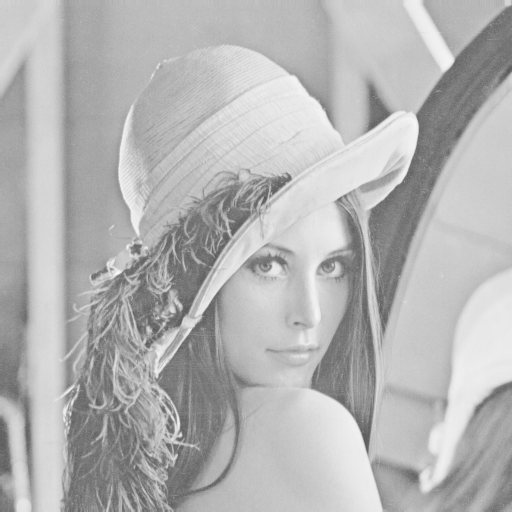
\includegraphics[width=.3\linewidth]{\detokenize{figuras/quantization/Luminance_gray.png}}
    \label{fig:luminance}
  }
  \subfloat[Luma]{
    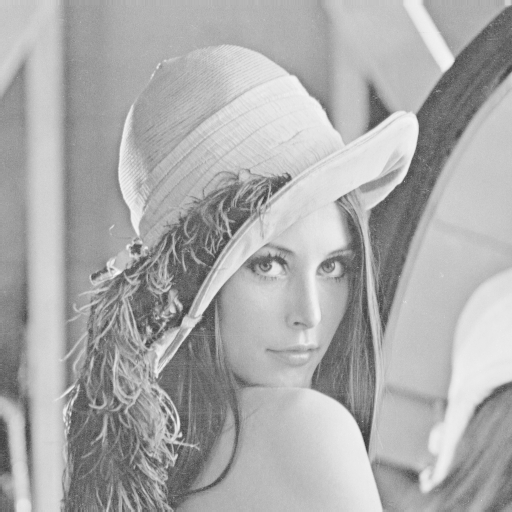
\includegraphics[width=.3\linewidth]{\detokenize{figuras/quantization/Luma_gray.png}}
    \label{fig:luma}
  }
  \subfloat[MSB]{
    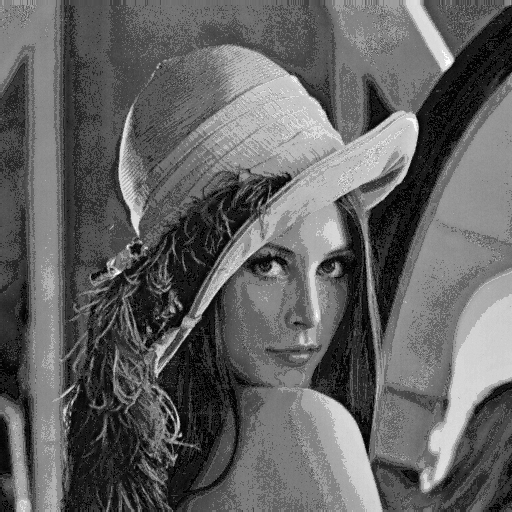
\includegraphics[width=.3\linewidth]{\detokenize{figuras/quantization/MSB_gray.png}}
    \label{fig:msb}
  }
   \end{center}
  %  \caption{Conversão para a escala de cinza com os métodos utilizados nessa pesquisa. Os métodos resultam em uma imagem com 8 bits (256 cores). \\ \textit{Fonte:~Elaborado pela autora.}}
  %  \label{fig:quantizacao}
  \end{figure}
\end{frame}
%-----------------------------------------------------------------------------
\subsection{Desbalanceamento de classes}
\begin{frame}{Desbalanceamento de classes}
\begin{figure}
    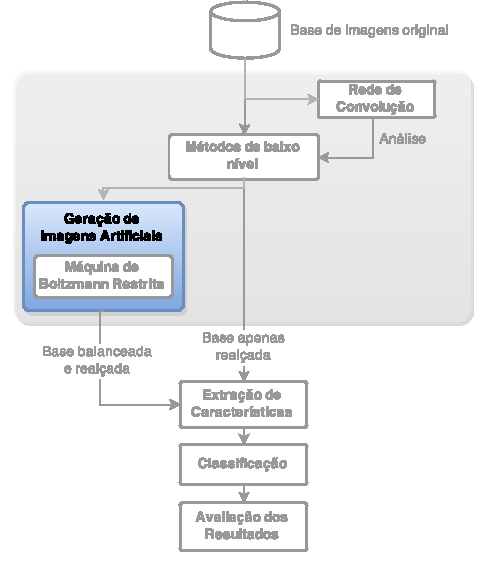
\includegraphics[height=0.75\textheight]{figuras/geral_geracao.pdf}
\end{figure}
\end{frame}
%-----------------------------------------------------------------------------
\begin{frame}{Desbalanceamento de classes}
\setstretch{1.2}
\setlength\leftmargini{0em}
\justifying
\setstretch{1.2}
\begin{itemize}
  \item Número desbalanceado de exemplos. Majoritárias x minoritárias.
  \item Abordagens:
    \begin{itemize}
        \item \emph{Modificar métodos de aprendizagem:} adicionar funções de custo na classificação;
        \item \emph{Pré-processamento ao reamostrar os dados:}
      \begin{itemize}
          \item Aumentar a minoritária;
          \item Diminuir a majoritária.
      \end{itemize}
    \end{itemize}
\end{itemize}
\end{frame}
%-----------------------------------------------------------------------------
\begin{frame}{Desbalanceamento de classes - Subamostragem}
\setlength\leftmargini{0em}
\justifying
    \begin{itemize}
        \item Diminuir o número de elementos do conjunto;
        \item Podem remover informações essenciais dos dados originais;
        \item Eliminar elementos distantes da fronteira de decisão;
        \item Normalmente apresentam resultados piores.
        % \item Não há melhor para todos os cenários.
    \end{itemize}
\end{frame}
%-----------------------------------------------------------------------------
\begin{frame}{Desbalanceamento de classes - Sobreamostragem}
\setlength\leftmargini{0em}
\justifying
    \begin{itemize}
        \item Aumentar o número de elementos;
    \begin{block}{SMOTE}
\setlength\leftmargini{1em}
        \begin{itemize}
            \item Multiplica a diferença entre o vetor de características de um elemento e do seu vizinho mais próximo por um número $0 \leq x \leq 1$;
            \item Adiciona ao vetor original, criando um novo elemento entre os dois vetores originais;
            \item Aprendido como exemplo da classe minoritária;
            \item Força uma região de decisão maior e mais geral;
        \end{itemize}
    \end{block}
    \end{itemize}
\end{frame}
%-----------------------------------------------------------------------------
\begin{frame}{Desbalanceamento de classes - SMOTE}
\setlength\leftmargini{0em}
\justifying
 \begin{figure}[hbpt]
 \begin{center}
   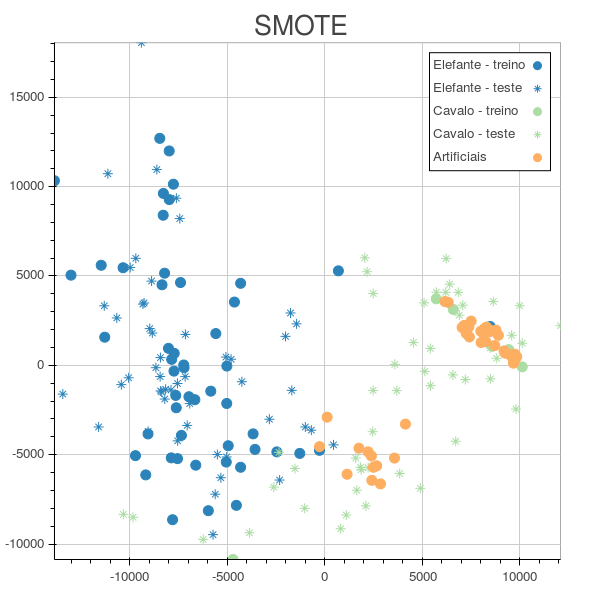
\includegraphics[width=.6\linewidth]{{figuras/smote.png}}
   % http://www.intechopen.com/books/advances-in-data-mining-knowledge-discovery-and-applications/selecting-representative-data-sets
 \end{center}
\end{figure}
\justifying
    \begin{itemize}
        \item Rebalancear ao gerar novos elementos, ao invés de replicá-los;
        \item Sobre os vetores de características previamente extraídos;
        \item (Chawla et al., 2002) \textbf{Diferentes estratégias para criar exemplos sintéticos podem melhorar a performance da classificação;}
        \item Utilizado para comparação.
    \end{itemize}
\end{frame}
%-----------------------------------------------------------------------------
\subsection{Extração de características}
\begin{frame}{Extração de Características}
\begin{figure}
    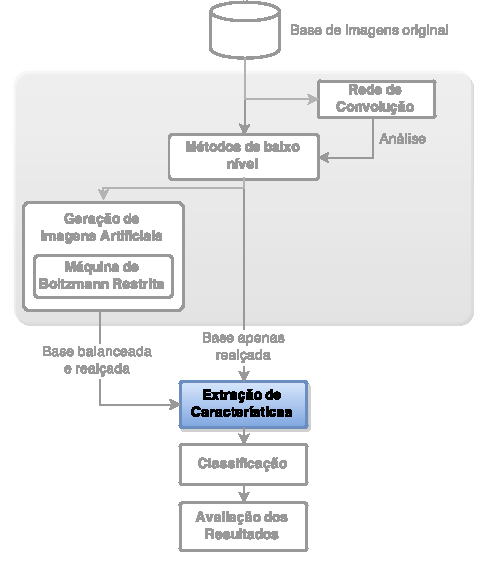
\includegraphics[height=0.75\textheight]{figuras/geral_extracao.pdf}
\end{figure}
\end{frame}
%-----------------------------------------------------------------------------
\begin{frame}{Extração de Características}
\setlength\leftmargini{0em}
\justifying
\begin{itemize}
\item Descrever as informações visuais relevantes em um vetor de características;
\item Entrada para o classificador de padrões;
% Exemplo: importante para a discriminação entre classes de algas é a forma.
\item Salientar as diferenças entre imagens de classes distintas e suavizar possíveis diferenças de imagens da mesma classe (Ex. algas - forma).
\end{itemize}
\setlength\leftmargini{0em}
\begin{description}
\item [Textura:] suavidade, aspereza e uniformidade. Ex. entropia;
\item [Forma:] características externas. Ex. curvatura;
\item [Cor:] distribuição espacial de cores na imagem. Ex. histograma.
\end{description}
\end{frame}
%%%%%%%%%%%%%%%%%%%%%%%%%%%%%%%%%%%%%%%%%%%%%%%%%%%%%%%%%%%%%%%%%%%%%%%%%%%%%%%
\section{Quantização de imagens}
\begin{frame}{Quantização de imagens}
\setstretch{1.2}
\setlength\leftmargini{1em}
\begin{block}{}
\justifying
\begin{itemize}
\item
\end{itemize}
\end{block}
\end{frame}
%%%%%%%%%%%%%%%%%%%%%%%%%%%%%%%%%%%%%%%%%%%%%%%%%%%%%%%%%%%%%%%%%%%%%%%%%%%%%%%
\section{Geração de imagens artificiais}
\begin{frame}{Geração de imagens artificiais}
\setstretch{1.2}
\setlength\leftmargini{1em}
\begin{block}{}
\justifying
\begin{itemize}
\item
\end{itemize}
\end{block}
\end{frame}
%-----------------------------------------------------------------------------
\begin{frame}{Metodologia - Implementação}
\setstretch{1.2}
\setlength\leftmargini{1em}
\begin{block}{}
\justifying
\begin{itemize}
\item Biblioteca OpenCV; %\cite{Intel2010}.
\item Linguagens de programação C++ e Python;
\item Código disponível em \footnotesize{\url{https://bitbucket.org/moacirponti/imagefeatureextraction/overview}}.
\end{itemize}
\end{block}
\end{frame}
%-----------------------------------------------------------------------------
\begin{frame}{Metodologia - Experimentos}
\setstretch{1.2}
\setlength\leftmargini{1em}
\begin{block}{}
\justifying
\begin{itemize}
\item Explorar algoritmos para evidenciar características relevantes:
\begin{itemize}
\item Melhorar discriminação entre as classes;
\item Auxiliar no rebalanceamento.
\end{itemize}
\item Entrada: imagens originais das coleções disponíveis na literatura;
\item Resultado: medidas estatísticas da classificação.
\end{itemize}
\end{block}
\end{frame}
%-----------------------------------------------------------------------------
\begin{frame}{Metodologia - Análise dos resultados}
\setstretch{1.2}
\setlength\leftmargini{1em}
\begin{block}{}
\justifying
\begin{itemize}
\item Comparar a classificação:
\begin{itemize}
\item Base original;
\item Base realçada pelo método proposto.
\end{itemize}
\item Comparar os métodos:
\begin{itemize}
\item Geração artificial;
\item Técnicas de sobreamostragem disponíveis na literatura, como o SMOTE.
\end{itemize}
\end{itemize}
\end{block}
\end{frame}
%-----------------------------------------------------------------------------
\begin{frame}{Metodologia - Avaliação da Classificação}
% \setstretch{1.2}
\setlength\leftmargini{1em}
\begin{block}{Medida F1}
\justifying
Problema da acurácia: minoritária sem resultados corretos. \\
% Performance da classificação em cenários desbalanceados.
\begin{itemize}

\item Precisão (exatidão): dos exemplos classificados como positivos, quantos realmente são.
\vspace{-1.5em}
\begin{equation*}
  P = \frac{VP}{VP + FP}
\end{equation*}
\item Revocação (completude): exemplos positivos corretamente classificados como tal.
\begin{equation*}
  R = \frac{VP}{VP + FN}
\end{equation*}

\pause
\begin{equation*}
  F1 = 2 \frac{P \cdot R}{P+R}
\end{equation*}
\end{itemize}
\end{block}
\end{frame}
%-----------------------------------------------------------------------------
\begin{frame}{Metodologia - Avaliação dos Vetores}
\setstretch{1.2}
\justifying
\setlength\leftmargini{1em}
\begin{block}{Mahalanobis}  %\cite{mahalanobis2000}

\begin{itemize}
\item Distância entre a média e a variância das classes;
\item Quanto maior a distância entre as distribuições das classes melhor;
\item Antes e depois dos processamentos a serem realizados.
\end{itemize}
\vspace{4pt}

Baseia na correlação entre as variáveis e pode ser definida por
\begin{equation*}
  D_m(x_i) = \sqrt{(x_i - \mu)C^{-1}(x_i-\mu)^T},
\end{equation*}
\noindent onde $x_i$ é um vetor de valores, $\mu$ a média e C a matriz de covariância.
\end{block}
\end{frame}
%-----------------------------------------------------------------------------
\begin{frame}{Metodologia - Avaliação}
\setstretch{1.2}
\setlength\leftmargini{1em}
\begin{block}{Teste de Friedman}
\begin{itemize}
\item Determinar se há diferença significante entre os resultados gerados;
\item Analisa as performances dos algoritmos e atribui um \textit{rank};
\item A hipótese nula a ser testada é que não há diferença estatística relevante entre as observações;
\item P-valor indica essa significância (limiar de 0,05).
\end{itemize}
\end{block}
\end{frame}
%%%%%%%%%%%%%%%%%%%%%%%%%%%%%%%%%%%%%%%%%%%%%%%%%%%%%%%%%%%%%%%%%%%%%%%%%%%%%%%
\section{Resultados}
%-----------------------------------------------------------------------------
\begin{frame}[plain]{Descrição do Experimento}
\begin{figure}[!htb]
 \begin{center}
   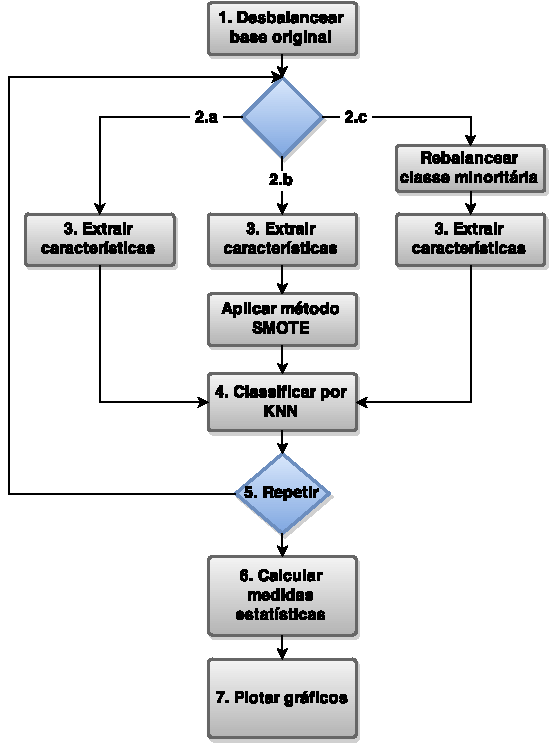
\includegraphics[width=0.65\textheight]{\detokenize {figuras/flow_main.pdf}}
 \end{center}
  \caption{Fluxo dos resultados preliminares.}
\end{figure}
\end{frame}
%-----------------------------------------------------------------------------
\begin{frame}[plain]{Descrição do Experimento}
\begin{figure}[!htb]
 \begin{center}
   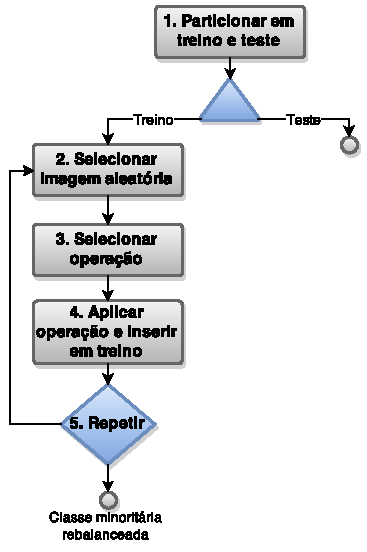
\includegraphics[width=0.55\textheight]{\detokenize {figuras/flow_sub.pdf}}
 \end{center}
  \caption{Fluxo da geração artificial.}
\end{figure}
\end{frame}
%-----------------------------------------------------------------------------
\begin{frame}{Descrição do Experimento}
\begin{itemize}
\item Classes praia e montanha da COREL-1000;
\item 50\% de teste/treino, com desbalanceamento da classe minoritária em 50, 25, 12 e 6;
\item \textbf{Geração artificial}: borramento, adição de ruído, realce, mistura e combinação;
\item \textbf{Quantização}: Intensidade para Haralick e MSB para os outros;
\item \textbf{Extração de características}: ACC, CCV, BIC, GCH e Haralick;
\item \textbf{Classificação} com KNN (K=1).
  % \begin{itemize}
  % \item Naive Bayes apresentou melhora com a replicação;
  % \item Comportamento não desejado para a avaliação do rebalanceamento de classes.
  % \end{itemize}
\end{itemize}
\end{frame}
%-----------------------------------------------------------------------------
\begin{frame}{Descrição do Experimento}
\setlength\leftmargini{0em}
\setstretch{1.2}
\justifying
Classes com alta sobreposição nas características de cor e textura.
\begin{figure}[!htb]
 \begin{center}
   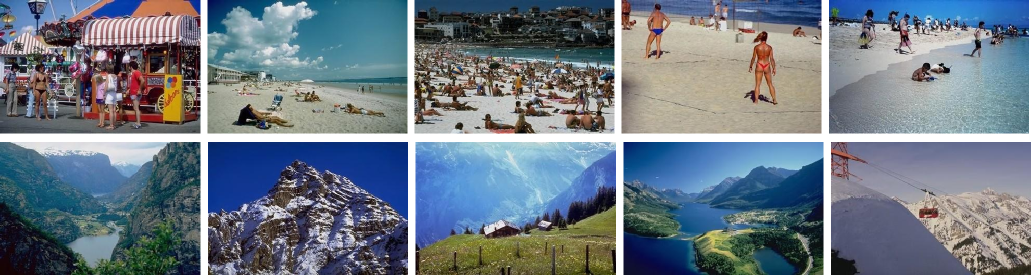
\includegraphics[width=\linewidth]{\detokenize{figuras/artificial-generation/2/praia-montanha.png}}
 \end{center}
\end{figure}
\end{frame}
%-----------------------------------------------------------------------------
\begin{frame}{Descrição do Experimento - Geração Artificial}
\setlength\leftmargini{1em}
\setstretch{1.2}
\renewcommand{\tabcolsep}{0.04cm}
\begin{figure}[!h]
\end{figure}
\renewcommand{\tabcolsep}{0.5cm}
\vspace{25pt}
\end{frame}
%-----------------------------------------------------------------------------
\begin{frame}{Descrição do Experimento - Extração de Características}
% \begin{frame}{Extração de Características}
\setlength\leftmargini{1.5em}
\begin{itemize}
\item[GCH]<1>
{\emph{Histograma global de cor} - $N$ (intensidades).} % Mais simples representação. }

\item[CCV]<2>
{\emph{Vetor de coerência de cor}. Classifica os pixels da imagem em coerentes e incoerentes de acordo com um \textit{threshold}, calcula e concatena os histogramas - $2N$.}

\item[BIC]<3>
{\emph{Classificação de pixels de borda e interior}. Mesma cor que seus vizinhos, é pixel de interior. Calcula dois histogramas - $2N$.}

\item[ACC]<4>
{\emph{Auto-correlograma de cor}: captura a correlação espacial entre cores idênticas. Probabilidade de encontrar dois pixels com a mesma cor, a uma distância $d$ um do outro. 1, 3, 5 e 7 - $4N$.}

\item[Haralick]<5>
{Entropia, homogeneidade, contraste, correlação, probabilidade máxima e uniformidade - $6$.}
\end{itemize}
\end{frame}
%-----------------------------------------------------------------------------
\begin{frame}{Resultados - Melhor Rebalanceamento}
\setlength\leftmargini{0em}
\justifying
\begin{itemize}
\item Ganho estatístico da medida-F, quando comparado à geração no espaço de atributos; % (ou seja, depois que as características já foram extraídas das imagens)
% \item Descritor ACC, conversão MSB e operação de pré-processamento combinação.
\end{itemize}
\vspace{-0.3cm}
\begin{figure}[htb]
 \begin{center}
  %  \includegraphics[width=0.7\linewidth]{\detokenize {figuras/4-ACC_MSB_FScore.png}}
 \end{center}
 \caption{Resultado obtido com a operação de combinação.}
\end{figure}
\end{frame}
%-----------------------------------------------------------------------------
\begin{frame}{Resultados - Pior Rebalanceamento}
\setlength\leftmargini{0em}
\setstretch{1.2}
\justifying
\begin{figure}[htb]
 \begin{center}
  %  \includegraphics[width=0.8\linewidth]{\detokenize {figuras/1-GCH_MSB_FScore.png}}
 \end{center}
 \caption{Piores resultados, obtidos com a adição de ruído.}
\end{figure}
% \begin{itemize}
% % \item Adição de ruído, extração com CCV e a quantização por MSB;
% \end{itemize}
\end{frame}
%-----------------------------------------------------------------------------
% \begin{frame}{Resultados}
% \setlength\leftmargini{0em}
% % \setstretch{1.2}
% \justifying
%
% \begin{itemize}
% \item Replicação: SRS - \textit{Simple Random Sampling};
% \item Não adiciona informações novas para o aprendizado.
% \end{itemize}
%
% \begin{figure}[htb]
%  \begin{center}
%    \includegraphics[width=0.65\linewidth]{\detokenize {figuras/resultado-copia.png}}
%  \end{center}
%   \caption{Simples replicação de exemplos sem pré-processamento.}
% \end{figure}
% \end{frame}
%-----------------------------------------------------------------------------
\begin{frame}{Resultados}
\setlength\leftmargini{0em}
\setstretch{1.2}
\justifying
\begin{itemize}
\item Melhores operações % : todas, apenas mistura e apenas composição;
% \item Piores: apenas borramento, ruído e \textit{unsharp masking} (filtros comuns);
% \vspace{2pt}
% \item Descritor que melhor se beneficiou: ACC;
% \item Descritores que não se beneficiaram: CCV e GCH;
% % \vspace{2pt}
% % \item Melhor quantizador: MSB;
% % \item Piores: CCV e GCH;
\end{itemize}
\end{frame}
%-----------------------------------------------------------------------------
\begin{frame}{Resultados}
\setlength\leftmargini{0em}
\setstretch{1.2}
\justifying
\begin{itemize}
\item Teste de Friedman para todas as execuções das melhores operações;
\item P-valor = $4.24E^{-11}$; Hipótese nula rejeitada.
\end{itemize}
\begin{table}[htb]
\centering
\caption{Posição média dos algoritmos utilizando Friedman}
  \begin{tabular}{c|c}
    Algoritmos  &   Posição \\ \hline
    Artificial  &   1.3863  \\
    Smote       &   1.6136  \\
    Original    &   3.0000  \\
  \end{tabular}
\end{table}
\begin{itemize}
\item Em algumas execuções: Artificial (1), SMOTE (2) e Original (3).
\end{itemize}
\end{frame}
%%%%%%%%%%%%%%%%%%%%%%%%%%%%%%%%%%%%%%%%%%%%%%%%%%%%%%%%%%%%%%%%%%%%%%%%%%%%%%%
\begin{frame}{Resultados - Rede de Convolução}
\begin{table}
\url{http://caffe.berkeleyvision.org/}
\caption{Treinamento das classes praia e montanha da base COREL-1000.}
  \begin{tabular}{c|c}
    Bases    &   Medida F1 \\ \hline
    Original não balanceada     &   0.708  \\
    Desbalanceada em 50\% &   0.577  \\
    Rebalanceada  &   0.677  \\
  \end{tabular}
\end{table}
\end{frame}
%%%%%%%%%%%%%%%%%%%%%%%%%%%%%%%%%%%%%%%%%%%%%%%%%%%%%%%%%%%%%%%%%%%%%%%%%%%%%%%
\begin{frame}{Artigo publicado na Neurocomputing}

\begin{columns}
  \begin{column}{0.5\textwidth}
  \centering
\begin{block}{}
\justifying
\tiny{
Ponti, M.; Nazaré, T; Thumé, G. \textbf{Image quantization as a dimensionality reduction procedure in color and texture feature extraction}, submitted to Neurocomputing, 2014.}
\end{block}
  \end{column}
  \begin{column}{0.5\textwidth}
  \centering
    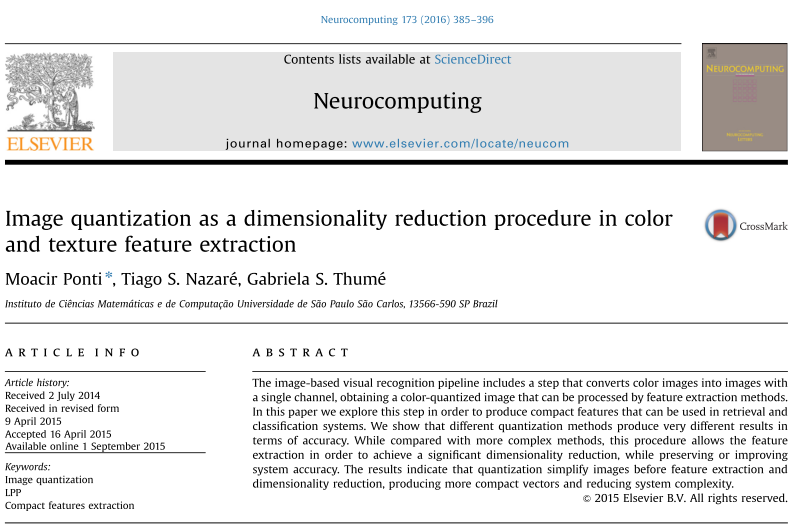
\includegraphics[width=0.9\linewidth]{figuras/artigo.png}
  \end{column}
\end{columns}
\end{frame}
%-----------------------------------------------------------------------------
\begin{frame}{Trabalhos futuros}
\setlength\leftmargini{0em}
\setstretch{1.2}
\justifying
  \begin{itemize}
  \item Analisar a memória associativa aprendida com uma máquina de Boltzmann restrita.
  \begin{itemize}
    \item Escolher para qual imagem original utilizar, ao invés do método aleatório utilizado nos resultados preliminares;
    \item Verificação da relevância das imagens geradas.
  \end{itemize}
  \end{itemize}
\end{frame}
%%%%%%%%%%%%%%%%%%%%%%%%%%%%%%%%%%%%%%%%%%%%%%%%%%%%%%%%%%%%%%%%%%%%%%%%%%%%%%%
\begin{frame}{Agradecimentos}
  Moacir Antonelli Ponti \\
  João do Espirito Santo Batista Neto \\

\centering{
  \begin{columns}
    \begin{column}{0.6\textwidth}
      \begin{figure}[!htbp]
        \begin{center}
        \subfloat{
          
\includegraphics[width=0.6\columnwidth]{figuras/cnpqLogo.jpg}
        }
        \newline
        \subfloat{
          
\includegraphics[width=0.4\columnwidth]{figuras/capesLogo.png}
        }
        \end{center}
      \end{figure}
    \end{column}
    \begin{column}{0.3\textwidth}
      
\includegraphics[width=\columnwidth]{figuras/brasao_usp_pb}
    \end{column}
  \end{columns}
}
\end{frame}
%-----------------------------------------------------------------------------
% \section{Referências}
\nocite{*}
%\section{Referências}
\begin{frame}[allowframebreaks]{Referências}
\tiny
% \bibliographystyle{apacite}
\bibliographystyle{plain}
%\bibliographystyle{amsalpha}
\bibliography{referencias}
\end{frame}

%-----------------------------------------------------------------------------
\begin{frame}[plain]
  \maketitle
\end{frame}
%%%%%%%%%%%%%%%%%%%%%%%%%%%%%%%%%%%%%%%%%%%%%%%%%%%%%%%%%%%%%%%%%%%%%%%%%%%%%%%%
\end{document}
